\section{原理}
\subsection{LabVIEW}
NATIONAL INSTRUMENTS(NI)が提供しているLabVIEWは,各種計測器やmyRIOなどを用いて自動計測や制御を実装するためのグラフィカルユーザーインターフェイスのプログラミング言語である.
主な特徴は,ビルトインされた仮想計測器(Virtual Instruments,以下VI)で,オシロスコープやマルチメーターなどの計測器と似た外観や機能をコンピューター上へ作成するというものである.
VIは,フロントパネル,ブロックダイアグラム,アイコン-コネクタという3つ主要素から構成される.
プログラミングは,ブロックダイアグラム上にアイコンを配置し,各アイコン間のコネクタをつなぐ形で行う.

\subsection{myRIO}
myRIOは,デュアルコアのARM Cortex-A9 リアルプロセッサとカスタマイズ可能なXilinx FPGA・アナログプロセッサの駆動するプログラミング言語には,LabVIEWを用いる.
LabVIEWとmyRIOを用いることにより,制御,ロボット,メカトロニクス,組込などを容易に実現することができる.

\subsection{myRIO ブレッドボードアクセサリ}
myRIOの拡張ポートに接続可能なブレッドボードアクセサリ.
myRIOの5V,3.3V,GND端子及びAnalog I/O,Digital I/Oの端子が,ブレッドボード上に結線した回路とヘッダにマッピングされている.
そのため,ブレッドボード上に結線した回路とヘッダとをジャンパ線で結線することにより,回路への入出力制御および計測がmyRIOを用いて容易に実行することができる.

\subsection{可変抵抗器(ポテンショメータ)\cite{23r234r2}}
可変抵抗器(Potentiometer)は抵抗値を変更できる抵抗器の一種で,機械的な位置の変化をアナログ電気信号に変換することができる.
つまみを回すことにより,\wfig{ALPS}のように抵抗体の長さが変化することにより,抵抗値の変更が可能となっている.

\begin{figure}[h]
\centering
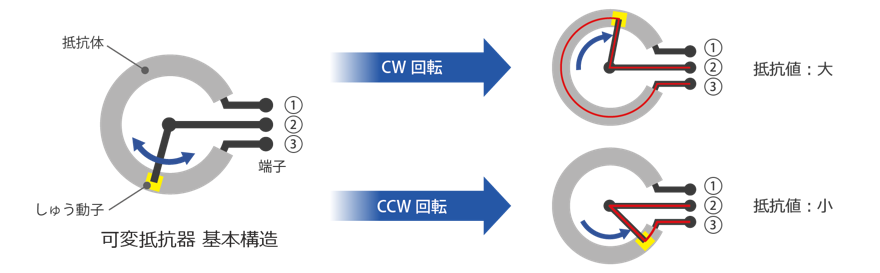
\includegraphics[scale=0.5]{/Users/ohyamasan/Downloads/TMCIT-Report/EE_Measurement/fig/pote_lp_01_02.png}
\caption{可変抵抗器の原理}
\label{fig:ALPS}
\end{figure}

\subsection{CdSセンサ\cite{dsfase}\cite{8347ty34i}\cite{B056}\cite{R300000001-I023994699-00}}
\label{CDSG}
光可変抵抗器ともいう.光電効果(photoelectric effect)である光導電性を利用し,光の強さで抵抗値が変化するCdS(硫化カドミウム)の性質を利用した電子部品.
光導電性は半導体の表面に光を当てるとキャリアが増加し,抵抗率が下がる現象である.
そのため,セルに当たる光が多ければ,抵抗値は低くなる.
赤外線や可視光線や紫外線など、広範囲の周波数にも反応するため,明るさセンサーや街の街灯のスイッチング等に用いられる.

\subsection{力センサ\cite{asdfsa}\cite{canon}}
\label{PG}
感圧センサともいう.
特殊導電部材(ゴム・フィルム)と電極で構成される.\wfig{weight}のように,接触の圧力に応じて特殊導電部材と電極の接触面積が増減することにより,抵抗値が変わる.センサ部分は円形などで,感圧エリアが決まっている.
圧力を加えていない時でも一定の抵抗値を有しており,圧力を加えると接触電極面が増加することから,抵抗値は減少する.

\begin{figure}[h]
\centering
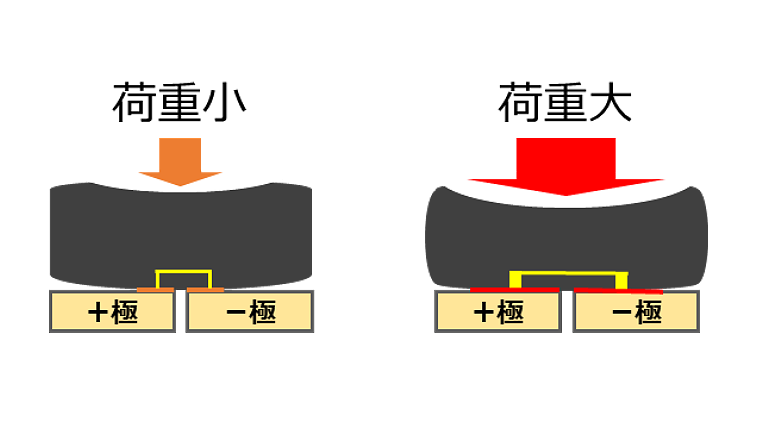
\includegraphics[scale=0.45]{/Users/ohyamasan/Downloads/TMCIT-Report/EE_Measurement/fig/sensor-03.png}
\caption{力センサの原理}
\label{fig:weight}
\end{figure}

\subsection{発光ダイオード\cite{dafadsav}\cite{gjkdgfbn}}
\label{LEDG}
LED(Light Emitting Diode)ともいう.
pn接合でできている.順方向の電圧を加えることにより,再結合エネルギーが光になって放出される.
電気エネルギーを直接光エネルギーに変換できるため,従来の光源と比べてエネルギー効率が高い.
白色LEDは\wfig{aokiro}のように,青色LED+黄色蛍光体(現在主流)のものと,\wfig{rgb}のように,赤色LED+緑色LED+青色LEDで作るものなどがある.

\begin{figure}[h]
  \begin{minipage}[]{0.5\hsize}
    \centering
    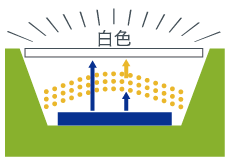
\includegraphics[scale=0.8]{/Users/ohyamasan/Downloads/TMCIT-Report/EE_Measurement/fig/led_what3_jp1.png}
    \caption{青色+黄色蛍光体手法}
    \label{fig:aokiro}
  \end{minipage}
  \begin{minipage}[]{0.5\hsize}
    \centering
    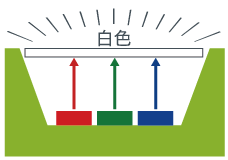
\includegraphics[scale=0.8]{/Users/ohyamasan/Downloads/TMCIT-Report/EE_Measurement/fig/led_what3_jp2.png}
    \caption{赤色+緑色+青色手法}
    \label{fig:rgb}
  \end{minipage}
\end{figure}


\subsection{真値と誤差及び相対誤差(誤差率)\cite{1130000797667922816}}
\subsubsection{真値(true value)}
真値とは,測定量(測定値ではない)が単位の何倍であるのかを示している値である.
真値は必ず存在すると仮定しても我々は真値そのものは知ることができず,ただその存在する範囲を推定することが出来るだけである.
そのため誤差は正負の符号を持っているが,それを確定することができない.
\subsubsection{誤差及び相対誤差}
測定値(measured value)及び,誤差(error)はそれぞれ,\weq{keisoku},\weq{gosa}で定義される.
\begin{align}
	測定値 &= 倍数 \times 単位\label{eq:keisoku}\\
	誤差 &= 測定値 − 真値\label{eq:gosa}
\end{align}
また,相対誤差(relative error)とは真値に対する誤差の比である.
但し真値は不明なことが多いため,通常は\weq{soutaigosa}のように誤差が小さいとして真値の代わりに測定値で割る.
\begin{eqnarray}
	相対誤差 = \frac{誤差}{真値} \fallingdotseq \frac{誤差}{測定値}
	\label{eq:soutaigosa}
\end{eqnarray}
相対誤差を百分率などで表した値を誤差率と呼ぶ.
また,以上のことから\weq{hutasikasa}のように表すこともできることがわかる\cite{1130000797042387712}.
\begin{eqnarray}
	測定値=真値 \pm 誤差=真値(1\pm 相対誤差)
\label{eq:hutasikasa}
\end{eqnarray}

\subsection{統計処理(正規分布・平均値・標準偏差)}
\subsubsection{正規分布(normal distribution)\cite{1130848328216058496}\cite{6602}}
左右対称の釣鐘型(平均値から離れるにつれて個数が減る)に値が分布している分布で,山の頂点に平均値がくる.
\wfig{normal-fig}は横軸に測定量,縦軸に正規分布の確率密度関数(probability density function)をプロットしたものである.
全体の面積(全確率)は\weq{int-nor}より1である.

\begin{figure}
\centering
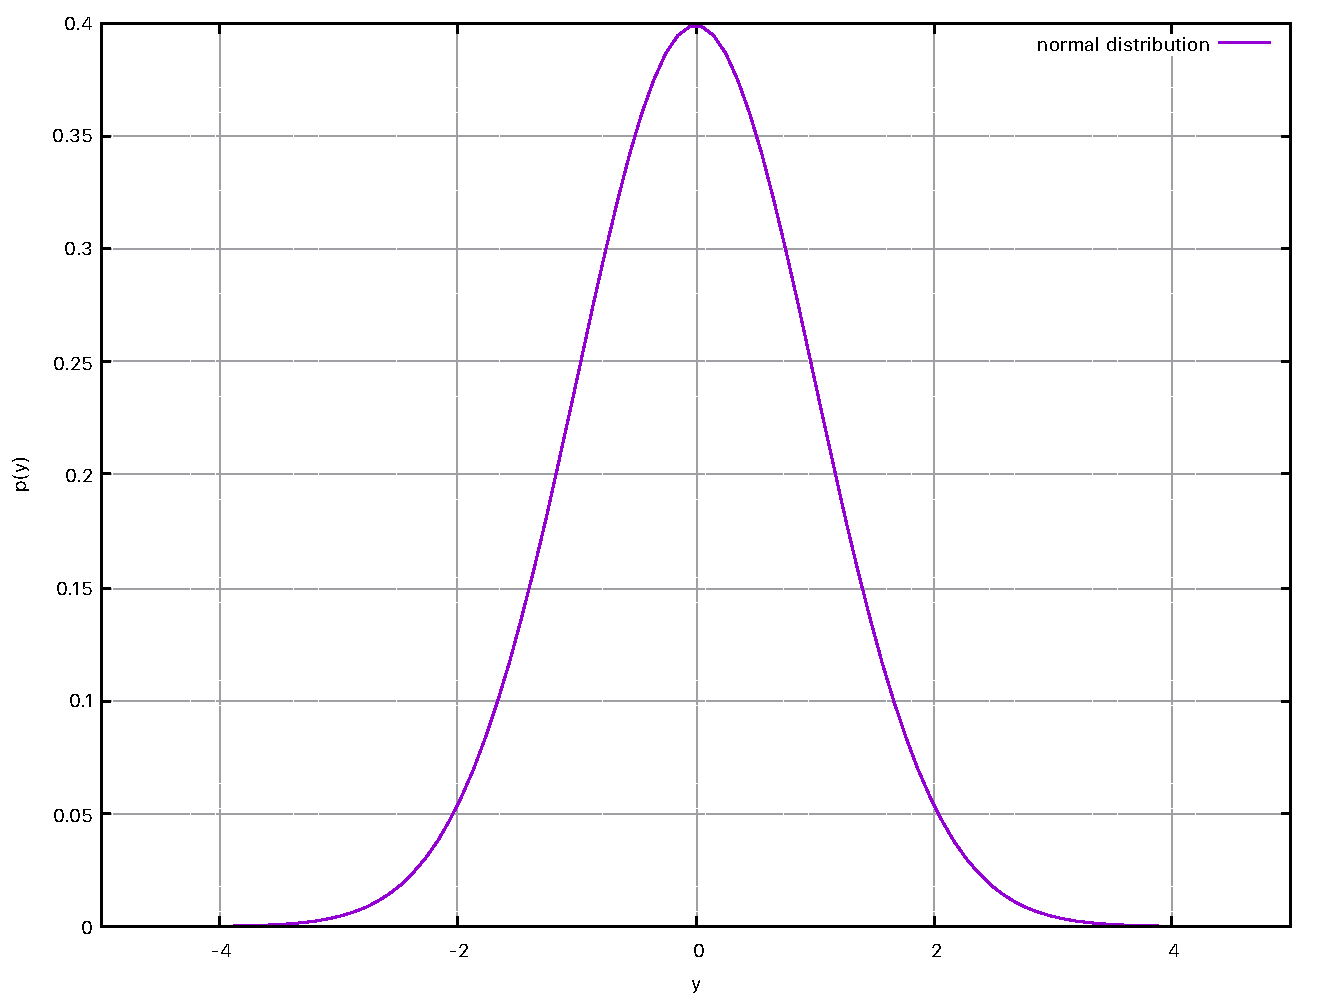
\includegraphics[scale=0.5]{/Users/ohyamasan/Downloads/TMCIT-Report/EE_Measurement/pre/plot.pdf}
\caption{正規分布}
\label{fig:normal-fig}
\end{figure}

\begin{equation}
\label{13}
p(x)=p(X=x)
\end{equation}

\begin{equation}
\label{eq:kakuritumitudo-fx}
p(x)=\frac{1}{\sqrt{2\pi}\sigma} \exp \left\{-\frac{(x-\mu)^2}{2\sigma^2}\right\}
\end{equation}

\begin{align}
\label{eq:int-nor}
\int_{-\infty}^{\infty} p(x)\,dx&=\frac{1}{\sqrt{2\pi}\sigma} \int_{-\infty}^{\infty} \exp \left(\frac{(x-\mu)^{2}}{2\sigma^{2}}\right)dx\nonumber\\
=&\frac{1}{\sqrt{2\pi}\sigma } \int_{-\infty}^{\infty} \exp \left(-\frac{y^{2}}{2\sigma^{2}}\right)dy\nonumber\\
=&\frac{1}{\sqrt{2\pi}\sigma }\sqrt{2\sigma^{2}\pi}=1
\end{align}

\subsubsection{平均値(mean)}
(算術)平均値とは$N$個全てのデータの総和を$N$個で割って得られる値で,\weq{heikinchi}で表すことができる\cite{1130848328216058496}.
\begin{equation}
	\bar{y} = \frac{1}{N}\sum^N_{i = 1}y_i
	\label{eq:heikinchi}
\end{equation}		

\subsubsection{標準偏差(standard deviation)\cite{1130000797042387712}}
標準偏差とは平均値を基準に各測定量がどれほどのばらついているかを定量的に表す値で,\weq{hyoujunhensa}で表すことができる.
\begin{equation}
	\sigma = \sqrt{\frac{1}{N - 1}\sum^N_{i = 1}(y_i - \bar{y})^2}
	\label{eq:hyoujunhensa}
\end{equation}	

\subsection{最小二乗法(method of least squares)\cite{1130848328216058496}\cite{1130282272174486912}}
2つの測定データ$y, x$間に一次方程式の関係があるとし,
\begin{equation}
	y = ax + b
	\label{eq:aiu}
\end{equation}
の傾き$a$,切片$b$を測定データからもっともらしい値にすることを考える.
その際に,
\begin{eqnarray}
	I &=& \sum\limits_{i=1}^{N} \varepsilon^2_i \nonumber\\
	&=& \sum\limits_{i=1}^{N} \bigl( y_i - f(x_i)\bigr)^2\nonumber\\\
	&=& \sum\limits_{i=1}^{N} \bigl( y_i - (ax_i+b)\bigr)^2
	\label{eq:error}
\end{eqnarray}
を最小にする$a$,$b$を求める.
これを最小二乗法といい,誤差を伴う測定値の処理においてその誤差の二乗の和を最小にすることで,最も確からしい関係式を求める方法である.前述の通り,誤差は正負あるため,2乘をしている.絶対値を用いると偏微分が不可能なため,平方根を用いた方法で行っている.
\begin{eqnarray}
	\frac{\partial}{\partial a}I(a,b) &=& 0\\
	\frac{\partial}{\partial b}I(a,b) &=& 0
\end{eqnarray}
から得られる方程式を,それぞれ$a$,$b$について解けば良く,それぞれの解を得るための方程式は次の2つを用いることになる.
\begin{equation}
	a = \frac{\sum_{n=1}^{n}(x_i -\bar{x})(y_i-\bar{y})}{\sum_{n=1}^{n}(x_i-\bar{x})^2}
	\label{eq:saisyou1}
\end{equation}
\begin{equation}
	b = \bar{y}-\frac{\sum_{n=1}^{n}(x_i -\bar{x})(y_i-\bar{y})}{\sum_{n=1}^{n}(x_i-\bar{x})^2} \bar{x}
	\label{eq:saisyou2}
\end{equation}
ここでは,\weq{aiu}のように1次式の形のものを示したが,一般に\weq{ippan}のような実験式に対して\weq{least-i}のように定義される.
\begin{align}
y&=F(x;a,b,c,\cdots)\label{eq:ippan}\\
(&xは変数,a,b,c,\cdots は定数)\nonumber
\end{align}
\begin{equation}
\label{eq:least-i}
I \equiv \sum_{i} (y_{i}-f(x_{i}))^{2} \quad \left(\frac{\partial I}{\partial a}=0 \to aを決定,\frac{\partial I}{\partial b}=0 \to bを決定 \cdots \right)
\end{equation}

